\documentclass{article}
\usepackage[a4paper,height=25cm,hmargin={2cm,2cm}]{geometry}
%<--------------------------------------------------------------------------->%
%%% Column %%%
\usepackage{multicol}  % \begin{multicols*}{3}[例外]字\end{multicols*}
\usepackage[english]{babel}
%<--------------------------------------------------------------------------->%
%%% Hyper Reference %%%
\usepackage[hidelinks]{hyperref}
%<--------------------------------------------------------------------------->%
%%% Math %%%
\usepackage{amsmath,amssymb}
\usepackage{mathrsfs,gensymb}
\usepackage{mathtools}
\DeclareMathOperator{\Exp}{\text{\textbf{E}}}
\DeclareMathOperator{\Var}{\text{Var}}
\newcommand{\E}[2][]{\Exp_{#1}[#2]}
\newcommand{\var}[2][]{\Var_{#1}[#2]}
\newcommand{\raum}{\phantom{=}{\:\,}}
\newcommand{\asDemonstrated}{\null\nobreak\hfill\ensuremath{\blacksquare}}
%<--------------------------------------------------------------------------->%
\newcommand{\T}{^{\mathsf{T}}}
\newcommand{\vv}{\mathbf{v}}
%<--------------------------------------------------------------------------->%
%%% TikZ %%%
\usepackage{tikz}
%<--------------------------------------------------------------------------->%
%%% Page # of # %%%
\usepackage{fancyhdr,lastpage}
\pagestyle{fancy}\renewcommand{\headrulewidth}{0pt}\fancyhf{}
\fancyfoot[C]{\footnotesize Page \thepage\ of \pageref{LastPage}}
\fancypagestyle{plain}{\renewcommand{\headrulewidth}{0pt}\fancyhf{}
\fancyfoot[C]{\footnotesize Page \thepage\ of \pageref{LastPage}}}
%<--------------------------------------------------------------------------->%
\title{What does it mean when we say\\``a covariance matrix is \textbf{bigger} than another''?}
\author{\texttt{jessekelighine.com}}
%<--------------------------------------------------------------------------->%

\begin{document}

\maketitle

\begin{multicols}{2}

\noindent
Consider two covariance matrices $A_{n\times n}$ and $B_{n\times n}$.
We say that $A$ is \textbf{bigger} than $B$,
often denoted by $A\geq B$ or $A\succeq B$, if $A-B$ is semi-positive definite.
Why do we use the ``definiteness'' of a matrix to compare the size of two covariance matrices?

First, notice that a covariance matrix is not only symmetrical, but also
semi-positive definite.  Consider a random vector $X=(X_1,...,X_n)\T$.
The covariance matrix is defined by
\begin{align*}
	K &\coloneqq \E{(X-\E{X})(X-\E{X})\T}.
\end{align*}
Given any constant vector $\vv$ of length $n$, we have
\begin{align*}
	\vv\T K \vv &= \E{\vv\T(X-\E{X})(\vv\T(X-\E{X}))\T} \geq 0
\end{align*}
by the definition of $K$.
Therefore, the covariance matrix $K$ is semi-positive definite.
(In fact, $\vv\T K\vv$ is zero iff $X$ has no variance at all.)

There is another intuitive way of interpreting the definiteness described above.
Consider the same vector $\vv$ and the random vector $X$.
The dot product $\vv\T X$ is the projection of the random vector from $n$-dimensional
space on a one-dimensional space along the direction of $\vv$, i.e.,
this collapse the $n$-dimensional random variable to a one-dimensional random variable through some linear combination.
If we calculate the variance of the one-dimensional random variable $\vv\T X$, we obtain
\begin{align*}
	\var{\vv\T X}
	&= \E{\vv\T X(\vv\T X)\T } - \E{\vv\T X}\E{\vv\T X}\T  \\
	&= \vv\T \big(\E{XX\T } - \E{X}\E{X}\T \big)\vv \\
	&= \vv\T K\vv.
\end{align*}
Notice that the variance assumes the exact form as before.
And since variance is non-negative, it is clear that the covariance matrix must be semi-positive definite.
That is, for any direction $\vv$,
the variance of ``$X$ projected on that direction'' is (clearly) non-negative.

Motivated by the intuitive interpretation,
let $X=(X_1,...,X_n)\T$ and $Y=(Y_1,...,Y_n)\T$ be random vectors with mean $(0,...,0)\T$ for simplicity.
Let $A=\E{XX\T}$ and $B=\E{YY\T}$ be the covariance matrices.
Our goal is to compare $A$ and $B$ in some meaningful way.
Since covariance matrices are multi-dimensional, it is not very straight forward.
However, we can project $X$ and $Y$ on a vector $\vv$,
an then compare the variance (non-negative real number) of the two projections.
To make the comparison meaningful,
it is reasonable to compare \emph{all} possible projections,
i.e., consider all possible choices of $\vv$.

Formally, consider any vector $\vv$.
The projection of $X$ on $\vv$ is $\vv\T X$.
The variance of $\vv\T X$ is 
\begin{align*}
	\E{(\vv\T X)^2}
	&= \E{\vv\T XX\T\vv} \\
	&= \vv\T\E{XX\T}\vv
	= \vv\T A\vv
\end{align*}
where $A$ is the covariance matrix.
Similarly, consider the same for $Y$.
If we find that $\forall\vv$,
\begin{align*}
	\vv\T A\vv - \vv\T B\vv
	= \vv\T (A - B)\vv
	\geq 0,
\end{align*}
then, by definition, $A-B$ is semi-positive definite.
Therefore, we define $A\geq B$ if $A-B$ is semi-positive definite.
The interpretation is that
``the variance of $X$ is larger than $Y$ in \emph{all directions}''.
(This is called the L\"{o}wner partial ordering.)

This interpretation of the partial ordering can be understood easily through visualisation.
The following are representations of the distributions $X$ and $Y$ where the
two random vectors are two-dimensional:
\begin{center}
	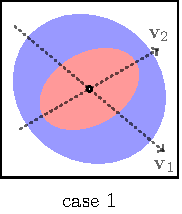
\includegraphics[width=0.2\textwidth]{figures/visual-1.pdf}
	\hspace{0.5em}
	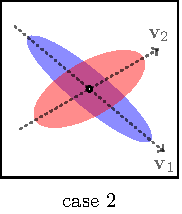
\includegraphics[width=0.2\textwidth]{figures/visual-2.pdf}
\end{center}
Let $X$ with covariance matrix $A$ be the blue distribution and $Y$ with
covariance matrix $B$ be the red distribution.
It is clear that in case 1, $A$ is \textbf{bigger} than $B$ since the variance of $X$ is
bigger that $Y$'s in \emph{every} direction. (every possible direction of projection)
However, the same statement is not true in case 2.
In some directions (e.g.\! $\vv_1$), the variance of $X$ is larger;
in other directions (e.g.\! $\vv_2$), the variance of $Y$ is larger.
Thus, $A$ and $B$ are not comparable by the partial order in case 2.
\asDemonstrated

\end{multicols}

\end{document}
